%%%%%%%%%%%%%%%%%%%%%%%%%%%%%%%%%%%%%%%%%
% Beamer Presentation
% LaTeX Template
% Version 1.0 (10/11/12)
%
% This template has been downloaded from:
% http://www.LaTeXTemplates.com
%
% License:
% CC BY-NC-SA 3.0 (http://creativecommons.org/licenses/by-nc-sa/3.0/)
%
%%%%%%%%%%%%%%%%%%%%%%%%%%%%%%%%%%%%%%%%%

%----------------------------------------------------------------------------------------
%	PACKAGES AND THEMES
%----------------------------------------------------------------------------------------

\documentclass[UTF8,aspectratio=169,14pt]{ctexbeamer}

\usepackage{hyperref}
\hypersetup{
	colorlinks=true,
	linkcolor=red,
	anchorcolor=blue,
	citecolor=green
}

\mode<presentation> {
	
	% The Beamer class comes with a number of default slide themes
	% which change the colors and layouts of slides. Below this is a list
	% of all the themes, uncomment each in turn to see what they look like.
	
	%\usetheme{default}
	%\usetheme{AnnArbor}
	%\usetheme{Antibes}
	%\usetheme{Bergen}
	%\usetheme{Berkeley}
	%\usetheme{Berlin}
	%\usetheme{Boadilla}
	%\usetheme{CambridgeUS}
	%\usetheme{Copenhagen}
	%\usetheme{Darmstadt}
	%\usetheme{Dresden}
	%\usetheme{Frankfurt}
	%\usetheme{Goettingen}
	%\usetheme{Hannover}
	%\usetheme{Ilmenau}
	%\usetheme{JuanLesPins}
	%\usetheme{Luebeck}
	\usetheme{Madrid}
	%\usetheme{Malmoe}
	%\usetheme{Marburg}
	%\usetheme{Montpellier}
	%\usetheme{PaloAlto}
	%\usetheme{Pittsburgh}
	%\usetheme{Rochester}
	%\usetheme{Singapore}
	%\usetheme{Szeged}
	%\usetheme{Warsaw}
	
	% As well as themes, the Beamer class has a number of color themes
	% for any slide theme. Uncomment each of these in turn to see how it
	% changes the colors of your current slide theme.
	
	%\usecolortheme{albatross}
	%\usecolortheme{beaver}
	%\usecolortheme{beetle}
	%\usecolortheme{crane}
	%\usecolortheme{dolphin}
	%\usecolortheme{dove}
	%\usecolortheme{fly}
	%\usecolortheme{lily}
	%\usecolortheme{orchid}
	%\usecolortheme{rose}
	%\usecolortheme{seagull}
	%\usecolortheme{seahorse}
	%\usecolortheme{whale}
	%\usecolortheme{wolverine}
	
	%\setbeamertemplate{footline} % To remove the footer line in all slides uncomment this line
	%\setbeamertemplate{footline}[page number] % To replace the footer line in all slides with a simple slide count uncomment this line
	
	%\setbeamertemplate{navigation symbols}{} % To remove the navigation symbols from the bottom of all slides uncomment this line
}

\usepackage{graphicx} % Allows including images
\graphicspath{{./figs/}}
\usepackage{booktabs} % Allows the use of \toprule, \midrule and \bottomrule in tables
\usepackage{longtable}
\usepackage{listings}
\usepackage{xcolor}
\lstset{numbers=left, %设置行号位置
	numberstyle=\tiny, %设置行号大小
	keywordstyle=\color{blue}, %设置关键字颜色
	commentstyle=\color[cmyk]{1,0,1,0}, %设置注释颜色
	frame=single, %设置边框格式
	escapeinside=``, %逃逸字符(1左面的键),用于显示中文
	%breaklines, %自动折行
	extendedchars=false, %解决代码跨页时,章节标题,页眉等汉字不显示的问题
	xleftmargin=2em,xrightmargin=2em, aboveskip=1em, %设置边距
	tabsize=4, %设置tab空格数
	showspaces=false %不显示空格
}
% Fonts
% \usepackage{libertine}
% \setmonofont{Courier}
\setCJKsansfont[ItalicFont=Noto Serif CJK SC Black, BoldFont=Noto Sans CJK SC Black]{Noto Sans CJK SC}

%\def\imagepath{./resources/graphics}
%\usepackage[imagepath=\imagepath]{ditaa}
%\graphicspath{ {\imagepath/} }


%\usepackage{pgfpages}
%\setbeameroption{show notes on second screen}
%%----------------------------------------------------------------------------------------
%	TITLE PAGE
%----------------------------------------------------------------------------------------

\title[第8讲]{第8讲 :全局页替换算法} % The short title appears at the bottom of every slide, the full title is only on the title page
\subtitle{第五节:FBR:访问频率置换算法}
\author{向勇、陈渝、李国良} % Your name
\institute[清华大学] % Your institution as it will appear on the bottom of every slide, may be shorthand to save space
{
	清华大学计算机系 \\ % Your institution for the title page
	\medskip
	\textit{xyong,yuchen,liguoliang@tsinghua.edu.cn} % Your email address
}
\date{\today} % Date, can be changed to a custom date


\begin{document}

\begin{frame}
\titlepage % Print the title page as the first slide
\end{frame}

%\begin{frame}
%\frametitle{提纲} % Table of contents slide, comment this block out to remove it
%\tableofcontents % Throughout your presentation, if you choose to use \section{} and \subsection{} commands, these will automatically be printed on this slide as an overview of your presentation
%\end{frame}
%
%%----------------------------------------------------------------------------------------
%%	PRESENTATION SLIDES
%%----------------------------------------------------------------------------------------
%----------------------------------------------
\begin{frame}[plain]
    \frametitle{内存抖动问题(thrashing)}
	\begin{columns}
		\begin{column}{.5\textwidth}
	
	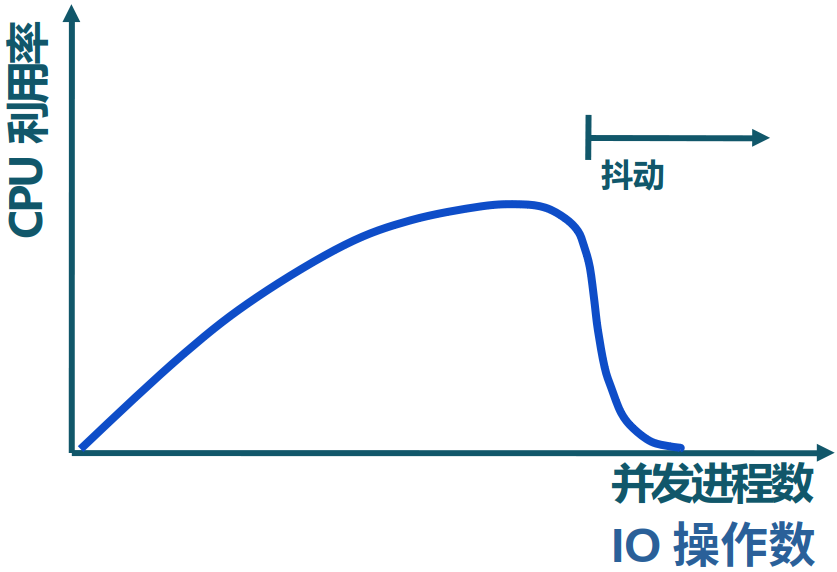
\includegraphics[width=1.\textwidth]{mem-trash}
	
\end{column}

		\begin{column}{.5\textwidth}
			
			%\begin{itemize}\Large
			%	\item 内存抖动问题(thrashing)
				\begin{itemize}\large
					\item 大量的IO访问
					\item 内存空间不够用
				\end{itemize}
			%\end{itemize}
			
		\end{column}
		

	\end{columns}
\end{frame}



%----------------------------------------------
\begin{frame}[plain]
	\frametitle{全局页面置换算法}
	\begin{columns}
		\begin{column}{.4\textwidth}
			\centering
			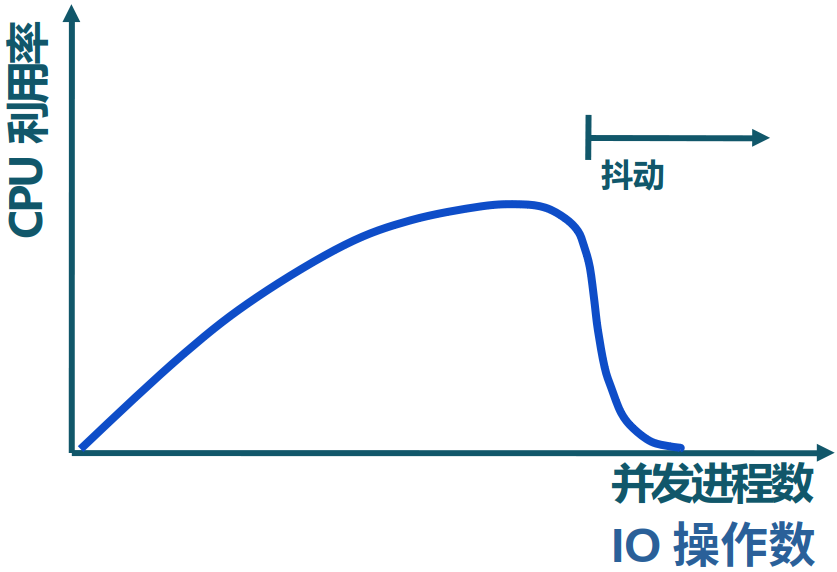
\includegraphics[width=.6\textwidth]{mem-trash}
			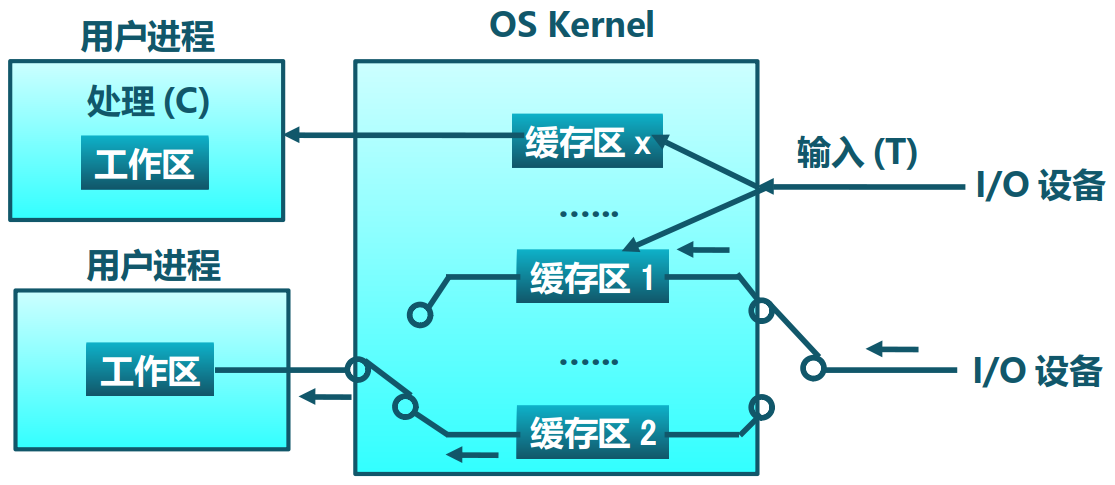
\includegraphics[width=1.2\textwidth]{buf-cache}
		\end{column}
		
		\begin{column}{.6\textwidth}
			
			%\begin{itemize}\Large
			%	\item 内存抖动问题(thrashing)
				\begin{itemize}\large
					%\item 全局页面置换算法
					\item 工作集算法:换出不在工作集中的页面
					\item 缺页率算法:使每个进程的缺页率保持在一个合理范围内
					\item LRU算法:选择最长时间没有被引用的页面进行置换
				\end{itemize}
			%\end{itemize}
			
		\end{column}
		
		
	\end{columns}
\end{frame}


%----------------------------------------------
% \begin{frame}[plain]
% 	\frametitle{ }
% 	\begin{columns}
% 		\begin{column}{.4\textwidth}
% 			\centering
% 			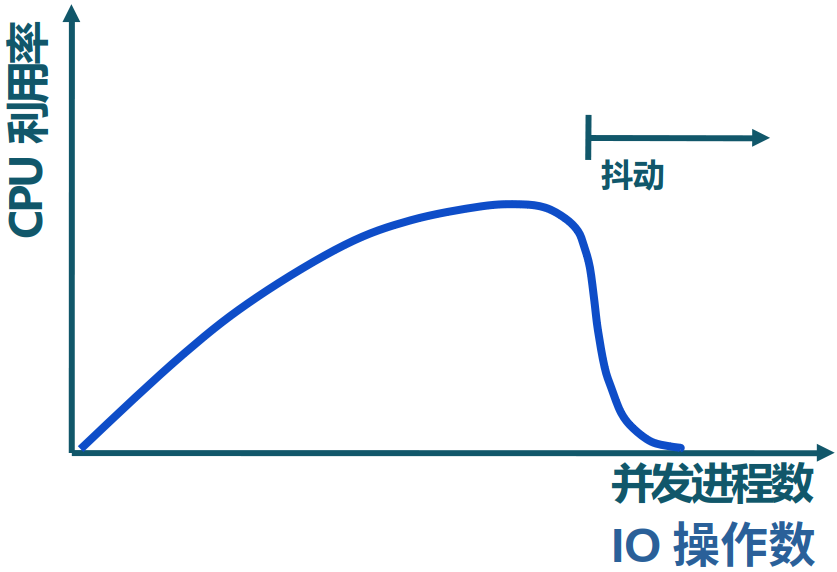
\includegraphics[width=.6\textwidth]{mem-trash}
% 			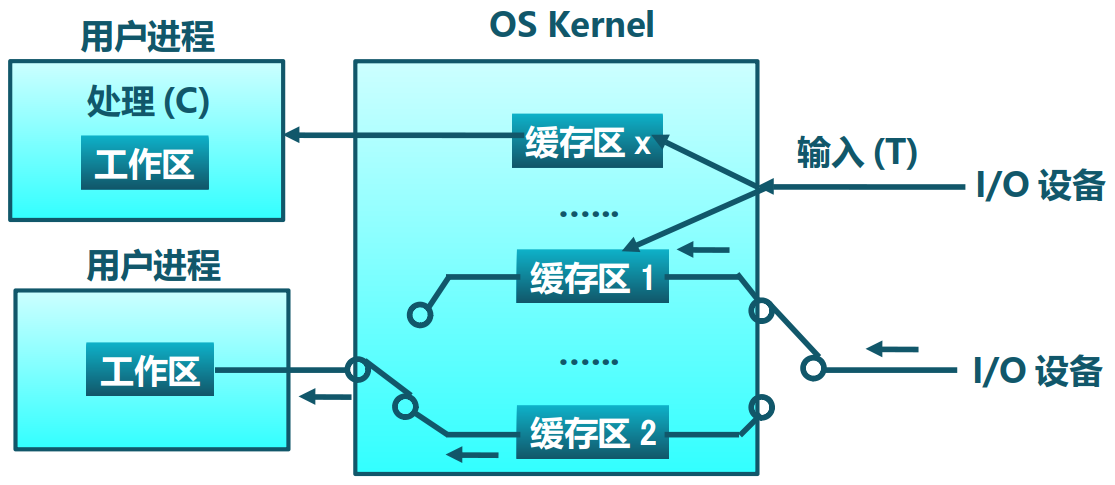
\includegraphics[width=1.2\textwidth]{buf-cache}
% 			
% %			缓存就是数据交换的缓冲区(称作Cache)。
% %			大部分的缓存使用,是为了提高程序数据的处理速度或者说提高程序的响应速度。 
% 		\end{column}
% 		
% 		\begin{column}{.6\textwidth}
% 			
% 			\begin{itemize}\Large
% 				\item LRU算法
% 				\begin{itemize}\large
% 
% 					\item 选择在内存驻留时间最长的页面进行置换
% 					\item 最优置换算法的一种近似
% 					\item 还有缺点与不足吗?
% 				\end{itemize}
% 			\end{itemize}
% 			
% 		\end{column}
% 		
% 		
% 	\end{columns}
% \end{frame}
% 
% 
%----------------------------------------------
\begin{frame}[plain]
	\frametitle{LRU算法的命中率}
	\begin{columns}
		\begin{column}{.4\textwidth}
			\centering
%			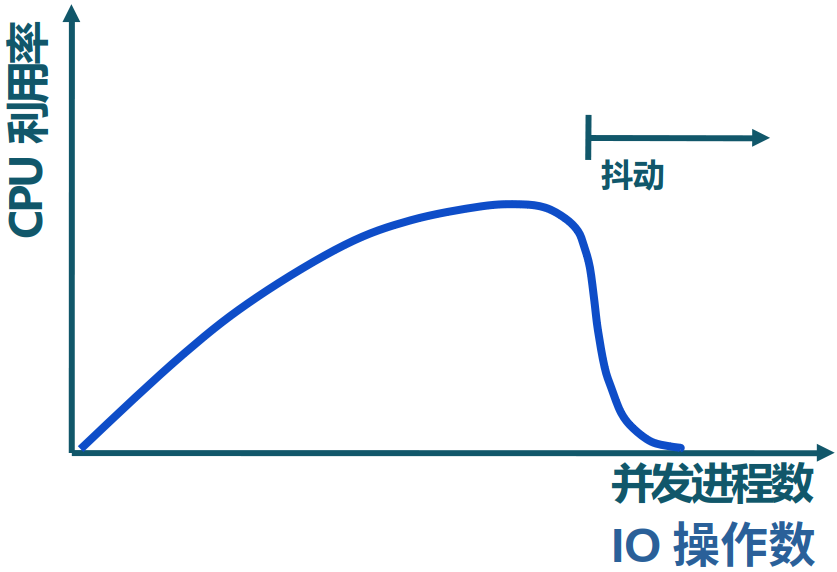
\includegraphics[width=.6\textwidth]{mem-trash}
			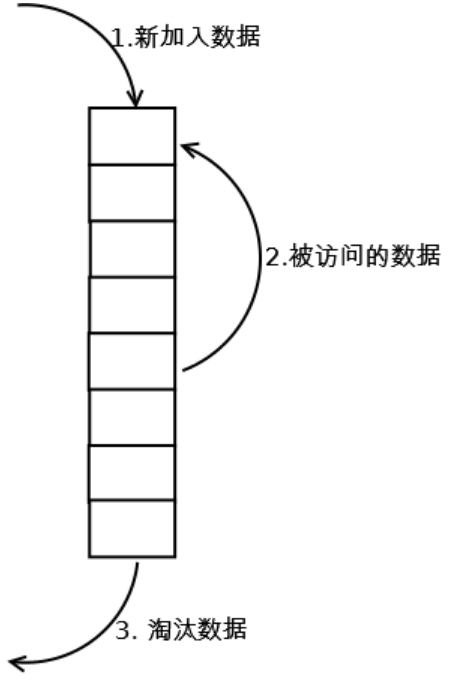
\includegraphics[width=.8\textwidth]{lru}
		\end{column}
		
		\begin{column}{.6\textwidth}
			
			%\begin{itemize}\Large
			%	\item LRU算法的命中率
				\begin{itemize}\large
					
					\item 当存在“热点”数据时,LRU的效率很好
					\item 但偶发性的、周期性的批量操作会导致LRU命中率急剧下降
					\item 缓存污染情况比较严重
					
				\end{itemize}
			%\end{itemize}
			\small
			缓存污染:是指OS将不常用的数据从内存移到缓存,造成常用数据的挤出,降低了缓存效率的现象。
		\end{column}
		
		
	\end{columns}
\end{frame}


%----------------------------------------------
\begin{frame}[plain]
	\frametitle{LRU算法的命中率}
	\begin{columns}
		\begin{column}{.5\textwidth}
			\centering
			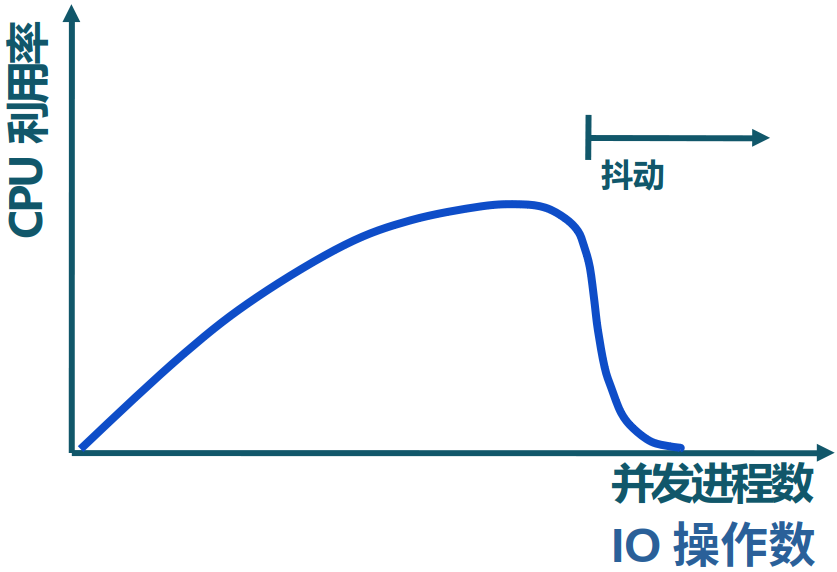
\includegraphics[width=.6\textwidth]{mem-trash}
			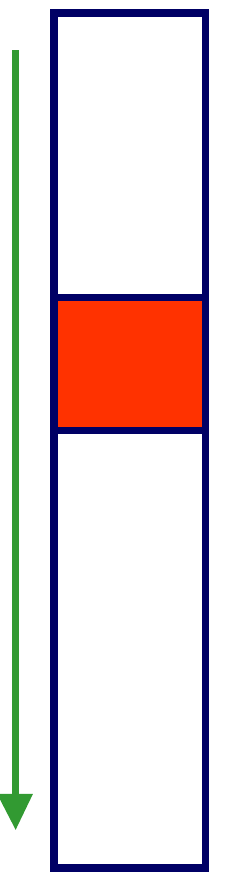
\includegraphics[width=.2\textwidth]{lru-badexample2}
			
		\end{column}
		
		\begin{column}{.5\textwidth}
			
			\begin{itemize}
				\item 多个运行程序访问客户记录的例子:LRU?
				\begin{itemize}
					\item 1,000,000个客户关系数据
					\item 大多数程序访问其中的一些红色部分(0.5\%)
					\item 个别程序批处理方式(绿线)访问整个客户关系数据
					
				\end{itemize}
			\end{itemize}
			
		\end{column}
		
		
	\end{columns}
\end{frame}

%----------------------------------------------
\begin{frame}[plain]
	\frametitle{LRU算法的命中率}
	\begin{columns}
		\begin{column}{.5\textwidth}
			\centering
			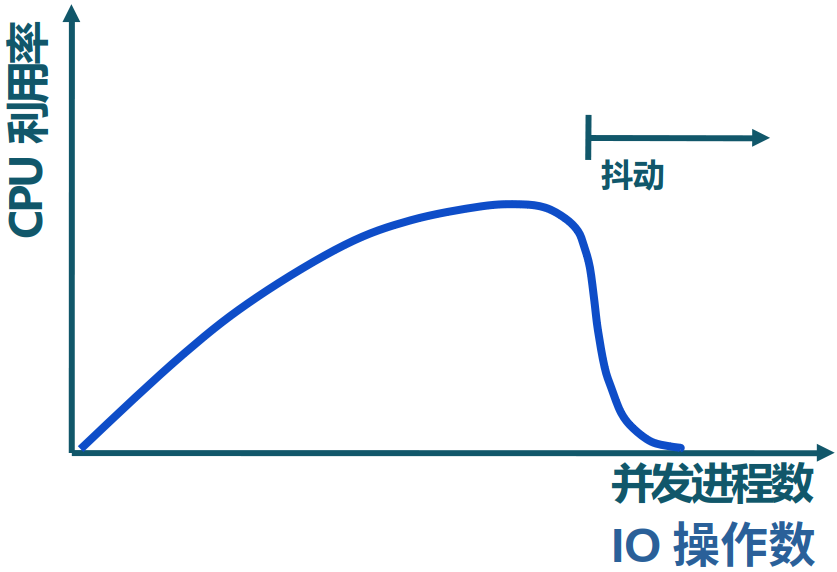
\includegraphics[width=.6\textwidth]{mem-trash}
			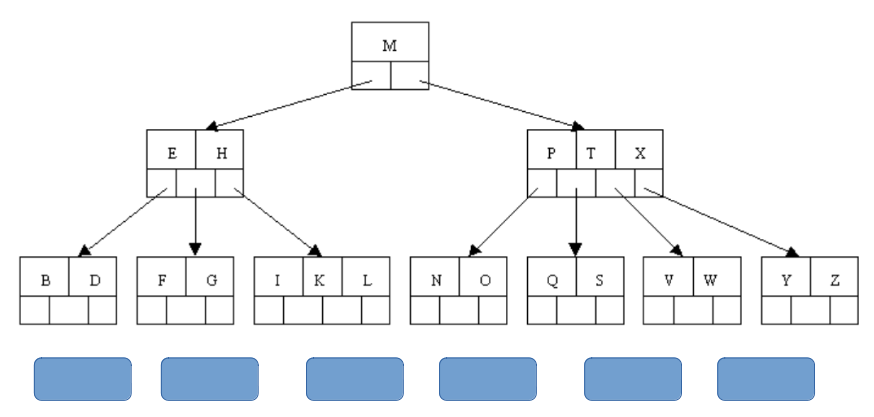
\includegraphics[width=1.2\textwidth]{btree}
		\end{column}
		
		\begin{column}{.5\textwidth}
			
			\begin{itemize}
				\item 一个程序访问客户记录的例子: LRU?
				\begin{itemize}
					
					\item 20,000个客户关系数据
					\item B-tree放置客户ID, 20Bytes/key
					\item 客户记录: 2000Bytes/record
					\item 100 pages for 客户ID
					\item 10,000 pages for 客户记录
					\item 共有101 pages, 4KBytes/page
					\item 访问模式: I1,R1,I2,R2,I3,R3...
					\item 访问概率: 客户ID pages 0.005
					\item 访问概率: 客户记录 pages 0.00005
				\end{itemize}
			\end{itemize}


		\end{column}
		
		
	\end{columns}
\end{frame}




%----------------------------------------------
\begin{frame}[plain]
	\frametitle{LRU算法的命中率}
	\begin{columns}
		\begin{column}{.5\textwidth}
			\centering
			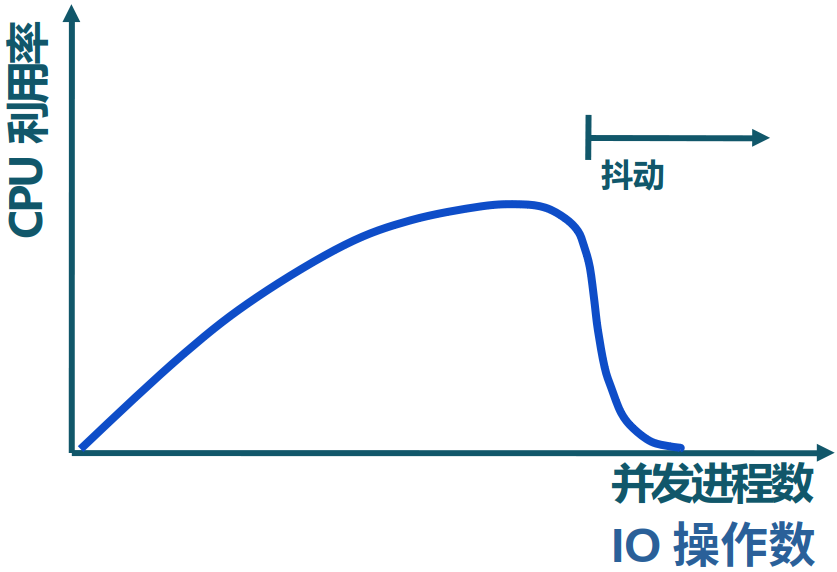
\includegraphics[width=.6\textwidth]{mem-trash}
			%			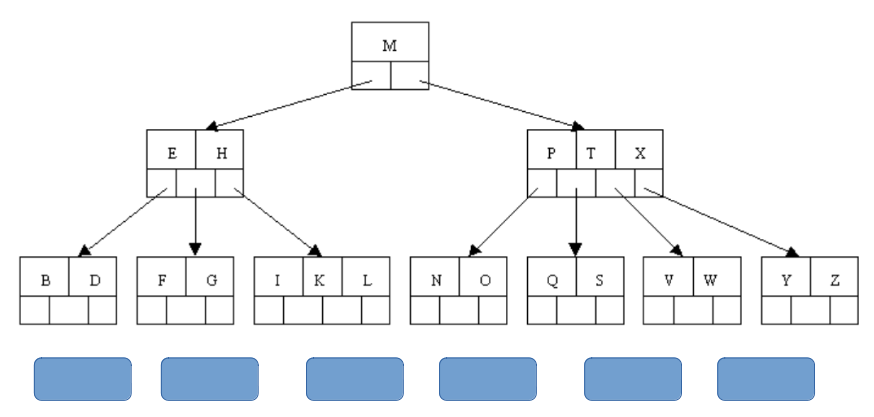
\includegraphics[width=1.2\textwidth]{btree}
		\end{column}
		
		\begin{column}{.5\textwidth}
			
			\begin{itemize}
				\item 为何LRU失效?
				\begin{itemize}
					
					\item 顺序块访问会把hot块替换出cache
					\item 对于索引块和数据块的循环访问时,不会根据访问概率缓存索引块
					
					\pause
					
					\item 完全从最近使用的时间角度考虑
					\item “最近使用过1次”
					\item 致命缺陷:就是没有考虑缓存单元的使用频率
				\end{itemize}
			\end{itemize}
			
			
		\end{column}
		
		
	\end{columns}
\end{frame}

%----------------------------------------------
\begin{frame}[plain]
	\frametitle{LFU算法的命中率}
	\begin{columns}
		\begin{column}{.5\textwidth}
			\centering
			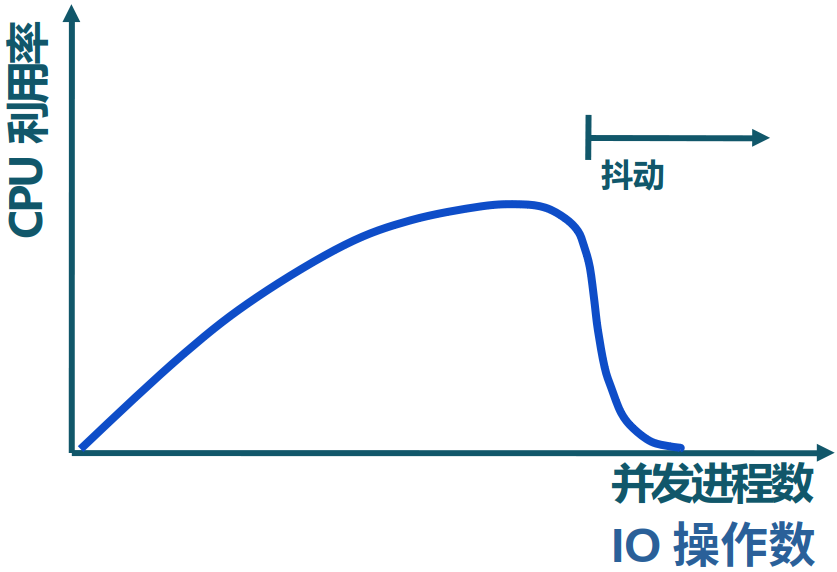
\includegraphics[width=.6\textwidth]{mem-trash}
			%			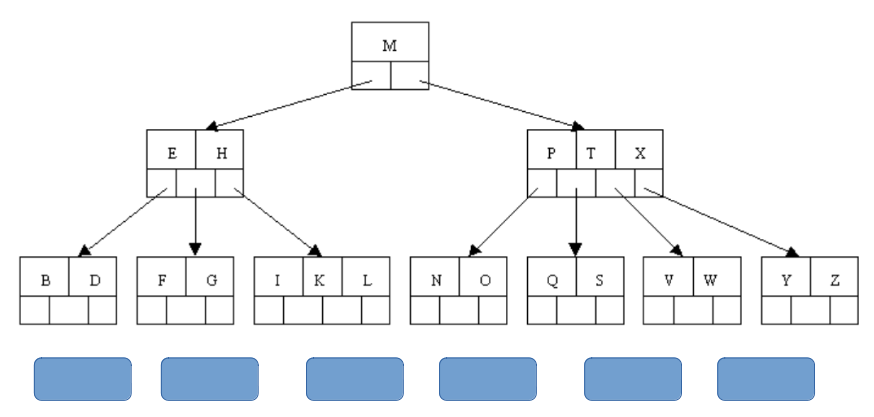
\includegraphics[width=1.2\textwidth]{btree}
		\end{column}
		
		\begin{column}{.5\textwidth}
			
			\begin{itemize}
				\item 为何LRU失效? 那LFU?
				\begin{itemize}
					
					\item   LFU(least frequently used): 淘汰使用频率最少的缓存单元
					
					\item 完全从使用频率的角度考虑
					\item 对最近的缓存单元的访问情况基本没考虑
					\item 对访问模式的改变基本上没有应变的策略

				\end{itemize}
			\end{itemize}
			
			
		\end{column}
		
		
	\end{columns}
\end{frame}

%----------------------------------------------
\begin{frame}[plain]
	\frametitle{访问频率置换算法(Frequency-based Replacement)}
	\begin{columns}
		\begin{column}{.1\textwidth}
			\centering
%			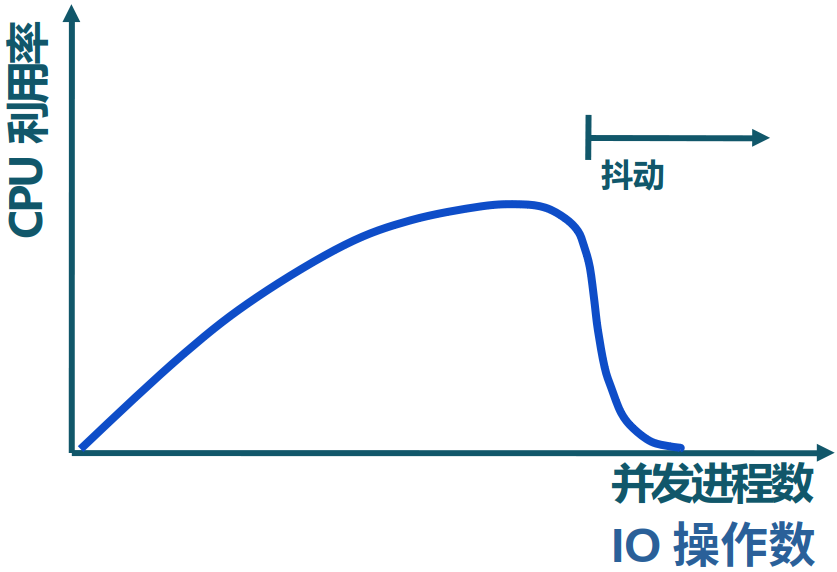
\includegraphics[width=.6\textwidth]{mem-trash}
			%			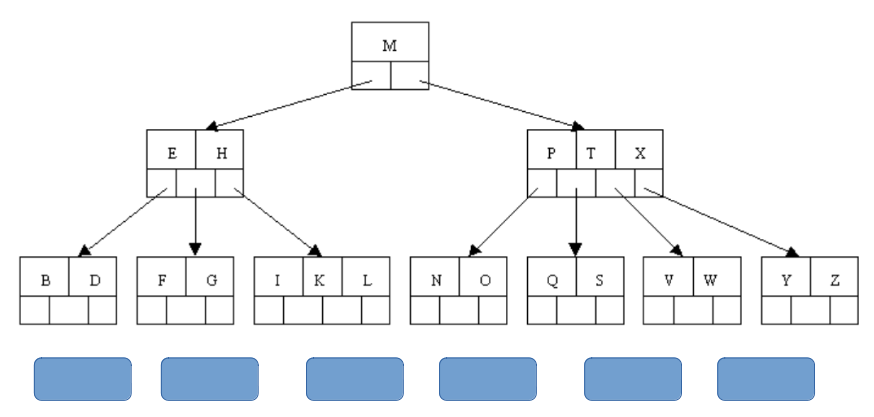
\includegraphics[width=1.2\textwidth]{btree}
		\end{column}
		
		\begin{column}{1.0\textwidth}
			
			\begin{itemize}
				\item LRU+LFU? 
				
				
				\begin{itemize}
					\item THE LEAST RECENTLY/FREQUENTLY USED (LRFU) POLICY?
					
					\item   在短周期中使用LRU算法,而在长周期中使用LFU算法?
					
					
				\end{itemize}
			\end{itemize}
			
			\tiny LRFU: A Spectrum of Policies that Subsumes the Least Recently Used and Least Frequently Used Policies  ,Donghee Lee,IEEE-TC 2001
		\end{column}
		
		
	\end{columns}
\end{frame}

%----------------------------------------------
\begin{frame}[plain]
	\frametitle{访问频率置换算法(Frequency-based Replacement)}
	\begin{columns}
		\begin{column}{.0\textwidth}
			\centering
			%			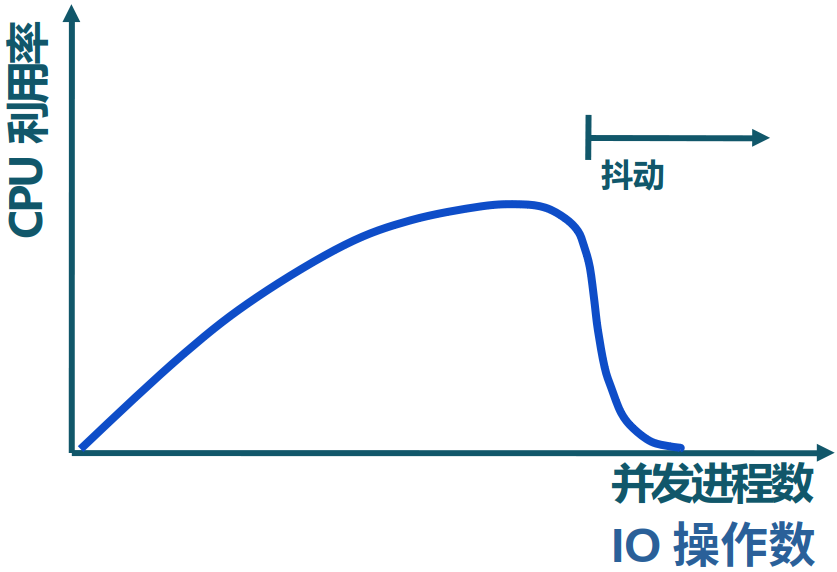
\includegraphics[width=.6\textwidth]{mem-trash}
			%			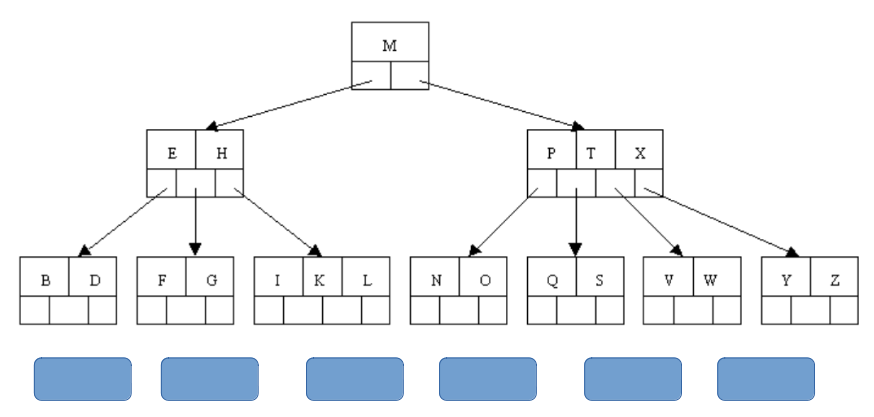
\includegraphics[width=1.2\textwidth]{btree}
		\end{column}
		
		\begin{column}{1.0\textwidth}
			
			\begin{itemize}
				\item LRU+LFU = FBR

			\end{itemize}
			
			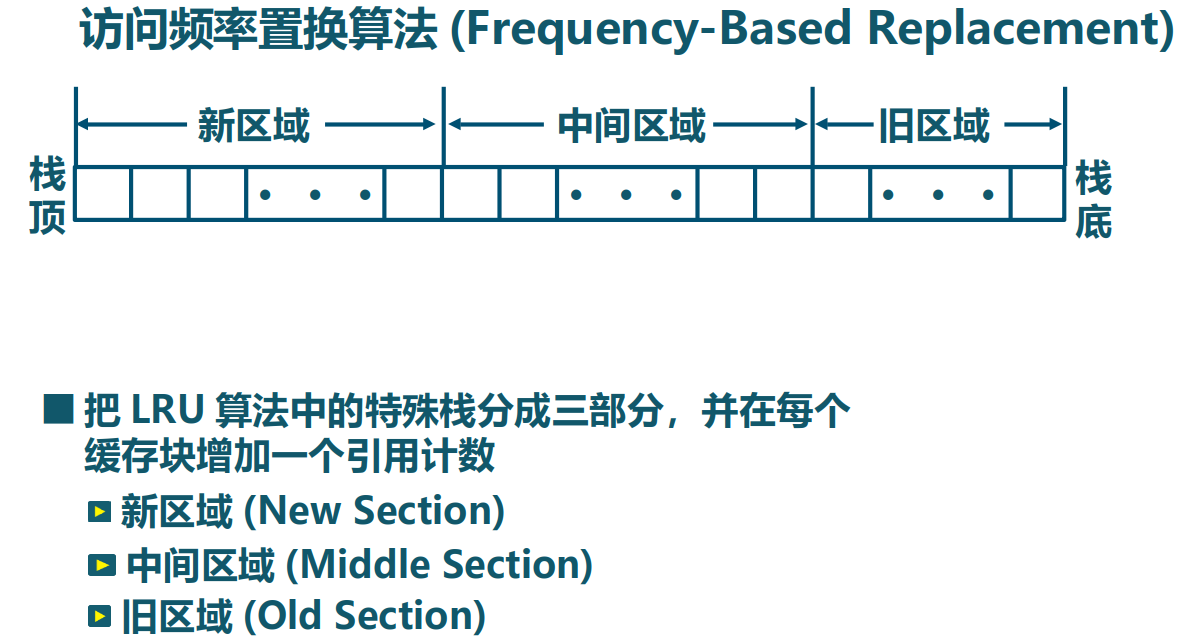
\includegraphics[width=.8\textwidth]{fbr}
		\end{column}
		
%		Data cache management using frequency-based replacement 
%		Authors:John T. Robinson,Murthy V. Devarakonda
%		SIGMETRICS '90: Proceedings of the 1990 ACM SIGMETRICS conference on Measurement and modeling of computer systemsApril 1990 Pages 134–142
	\end{columns}
\end{frame}


%----------------------------------------------
\begin{frame}[plain]
	\frametitle{访问频率置换算法(Frequency-based Replacement)}
	\begin{columns}
		\begin{column}{.0\textwidth}
			\centering
			%			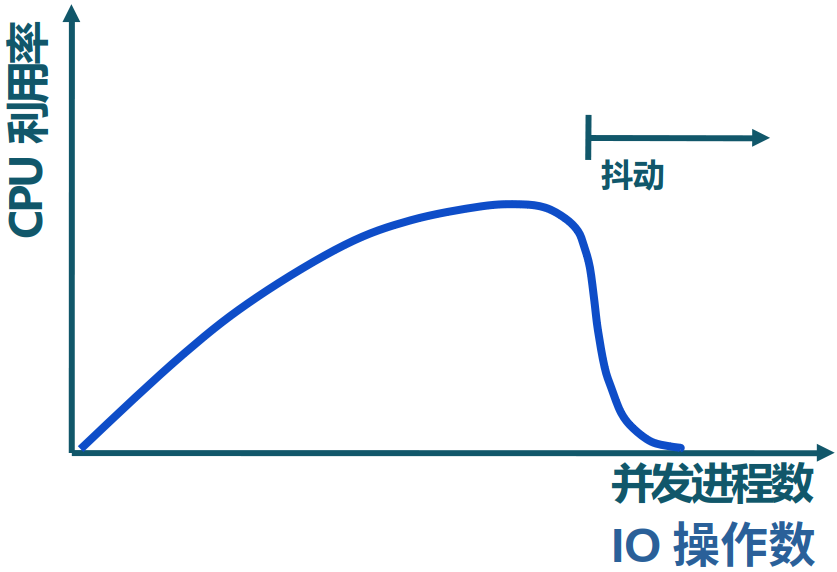
\includegraphics[width=.6\textwidth]{mem-trash}
			%			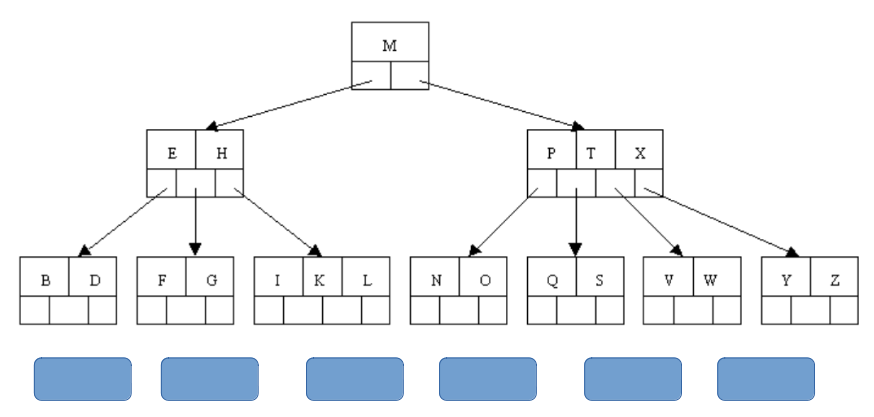
\includegraphics[width=1.2\textwidth]{btree}
		\end{column}
		
		\begin{column}{1.0\textwidth}
			
%			\begin{itemize}
%				\item LRU+LFU = FBR 访问频率置换算法(Frequency-based Replacement)
%				
%			\end{itemize}
			
			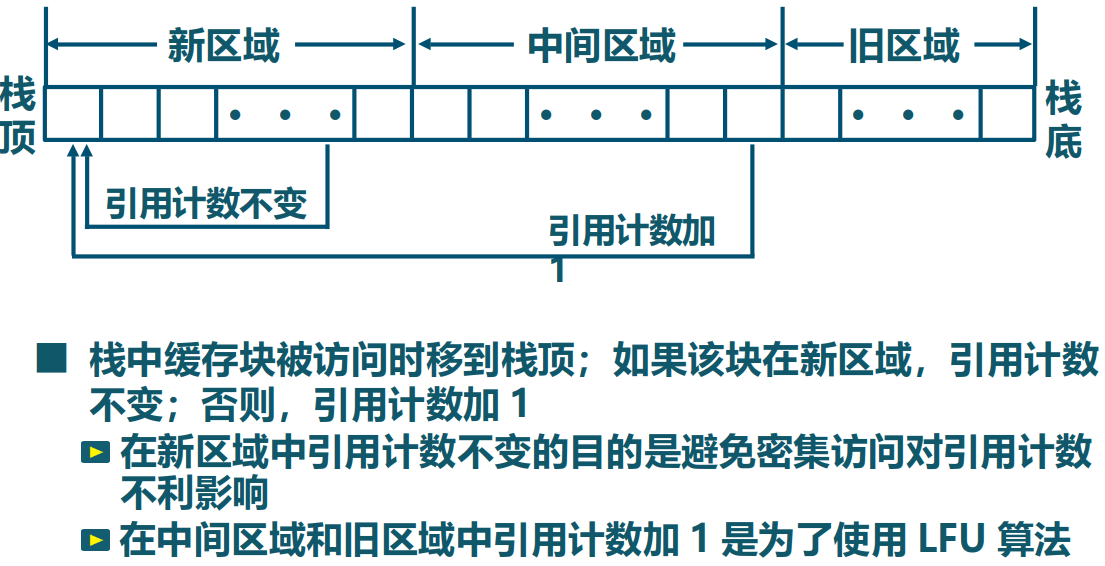
\includegraphics[width=.8\textwidth]{fbr2}
		\end{column}
		
		
	\end{columns}
\end{frame}



%----------------------------------------------
\begin{frame}[plain]
	\frametitle{ }
	\begin{columns}
		\begin{column}{.0\textwidth}
			\centering
			%			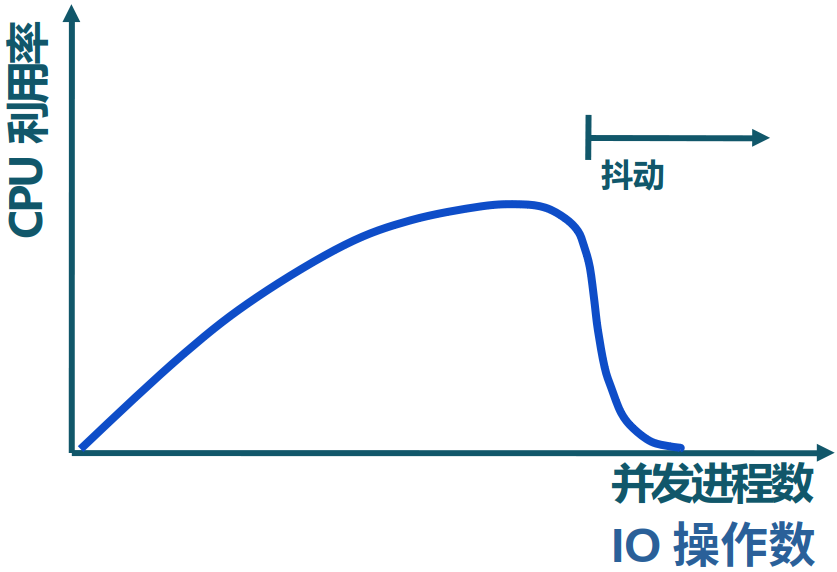
\includegraphics[width=.6\textwidth]{mem-trash}
			%			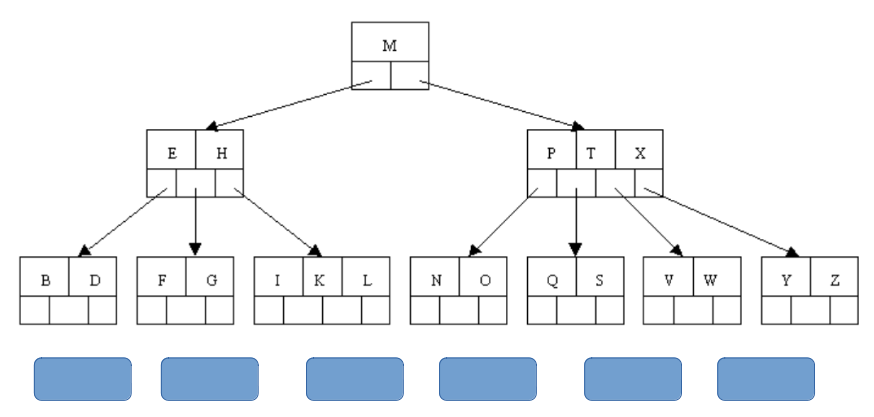
\includegraphics[width=1.2\textwidth]{btree}
		\end{column}
		
		\begin{column}{1.0\textwidth}
			
%			\begin{itemize}
%				\item LRU+LFU = FBR 访问频率置换算法(Frequency-based Replacement)
%				
%			\end{itemize}
			
			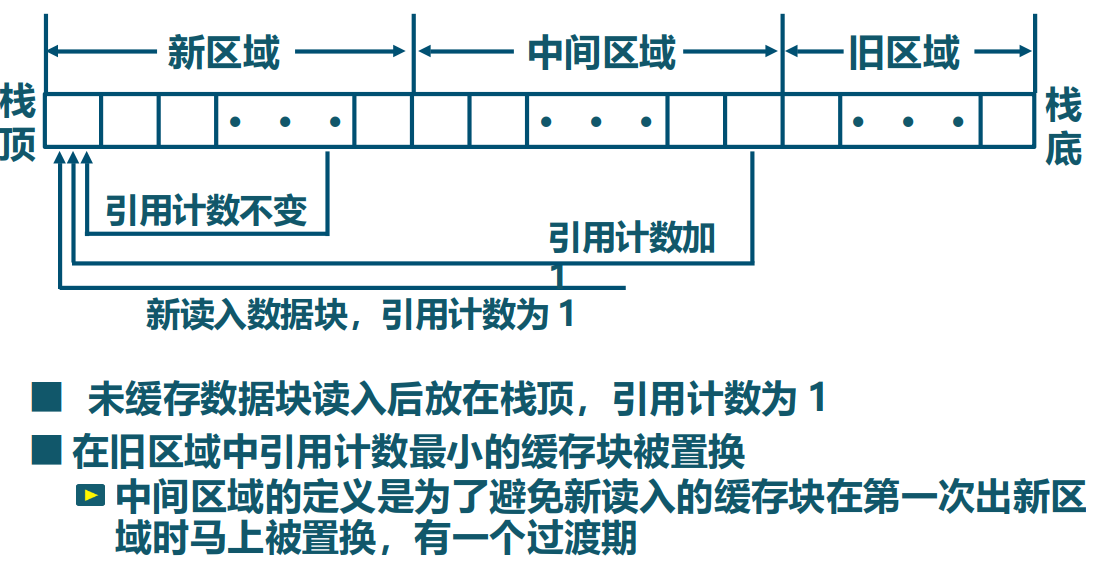
\includegraphics[width=.8\textwidth]{fbr3}
		\end{column}
		
		
	\end{columns}
\end{frame}



%----------------------------------------------
\begin{frame}[plain]
	\frametitle{访问频率置换算法(Frequency-based Replacement)}
	\begin{columns}
		\begin{column}{.0\textwidth}
			\centering
			%			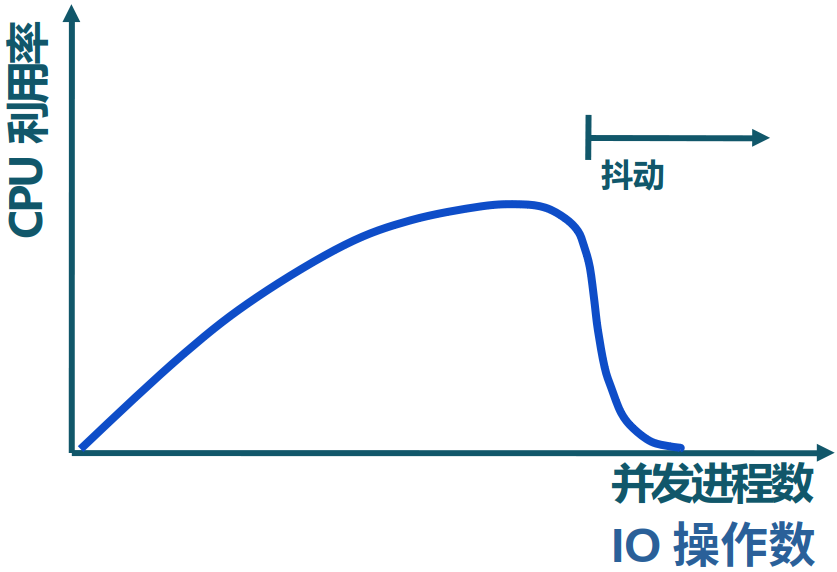
\includegraphics[width=.6\textwidth]{mem-trash}
			%			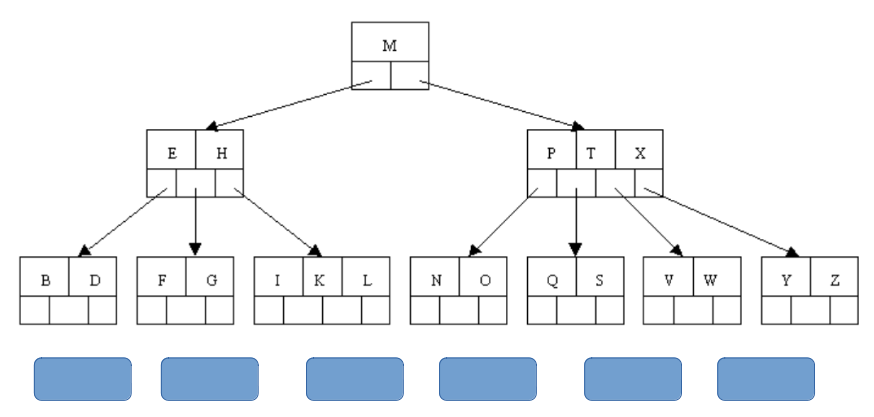
\includegraphics[width=1.2\textwidth]{btree}
		\end{column}
		
		\begin{column}{1.0\textwidth}
			
			\begin{itemize}
				\item FBR 访问频率置换算法的问题
				
					\begin{itemize}
					\item 需要可调参数:缓存中三块的大小,Cmax 和Amax
					\item 调整可调参数的时间周期
%					LRFU.pdf有讲Cmax 选择替换块的一个选择策略的阈值(zzz是smallest reference count block OR LRU block), Amax 用于调整 引用计数的一个阈值
				\end{itemize}
			\end{itemize}
			\centering
			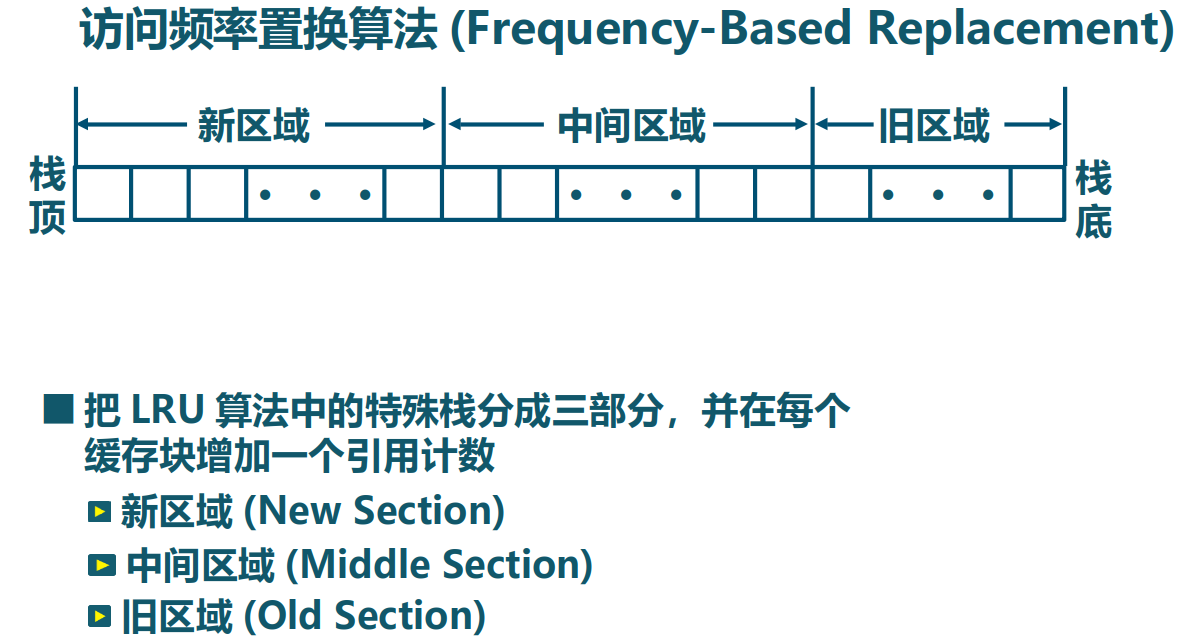
\includegraphics[width=.7\textwidth]{fbr}
		\end{column}
		
		
	\end{columns}
\end{frame}





%----------------------------------------------------------------------------------------

\end{document}
